\renewcommand{\labelitemi}{\textbullet}

\subsection{Consideraciones de diseño}
\begin{itemize}

	\item El TAD Pokemon es String porque asumimos que lo único que nos interesa saber es el tipo de pokemon. Asimismo, el TAD Jugador es Nat que se refiere a un ID único. El resto de los detalles relacionados (como sus posiciones, conexión del jugador, etc.) los maneja el TAD Sistema.

	\item Para el TAD Mapa el enunciado nos pide saber las posiciones válidas y como están conectadas entre sí, y para esto último supusimos que, además de saber si dos puntos están conectados, nos interesa saber si existe una conexión directa entre ellos (es decir, si hay un camino entre ambos sin otras posiciones en el medio)

	Por ejemplo, los siguientes casos se consideran distintos mapas (los puntos son posiciones y las líneas son conexiones directas):

	\bigskip
	\centerline{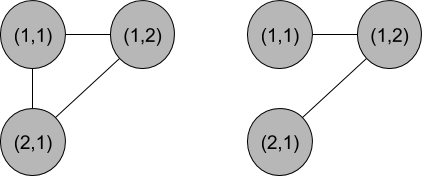
\includegraphics[scale=0.5]{nodos-mapa.png}}

	Cabe destacar que esto no afecta la lógica del juego, ya que los requisitos para movimientos válidos siguen siendo 1) una conexión (directa o no) y 2) distancia menor a 10, que se cumplen en ambos mapas. Por lo tanto, el movimiento de (1,1) a (2,1) y su inverso siempre son válidos.

	\item Cuando un jugador se registra, el mismo está desconectado y no tiene una posición inicial.

	\item Suponemos que un jugador puede estar en la misma posición que otros jugadores o un pokemon.

	\item Dado que el TAD Pokemon es String y no podemos diferenciar pokemons del mismo tipo, los \texttt{pokemonsCapturados} los representamos con un Multiconjunto de pokemons.

	\item La función \texttt{movsLejosDePos} tiene la logica de cuantos movimientos hubo fuera del rango de captura para avanzar la captura del pokemon que se ubica ahí. Asumimos que si 2 o más jugadores estan en el rango de captura de un pokemon determinado y uno de ellos sale del rango, este movimiento cuenta para los jugadores que permanecen en el rango.

	\item Extendimos los naturales para agregar la división y la raíz cuadrada. En ambos casos tomamos la parte entera y descartamos el resto.

	\item Extendimos el multiconjunto para agregarle la operación de partes, que genera un conjunto con todos los posibles subconjuntos del multiconjunto original.

\end{itemize}

\subsection{Consideraciones de reentrega}

\begin{itemize}

	\item Las funciones que corresponden a TADs preexistentes fueron movidas a extensiones de los mismos.

	\item Para solucionar la dependencia circular infinita y el comportamiento automático con capturaPokemon, modularizamos algunas funciones y agregamos \texttt{movsLejosDePosDespuesDelMov}. Así, podemos reducir la instancia sin problemas pero mantener el contador de 10 que teníamos antes.

	\item El generador \texttt{crearSistema} ahora toma la cotización inicial del sistema como parámetro.

	\item No se especifica en la consigna si pagarBoleta requiere que el jugador en cuestión esté conectado. Esto se puede modificar agregando la restricción \texttt{j $\in$ jugadoresConectados(jugadores(s), s)}.


\end{itemize}